% ==========================================================================
% INFO 4617 Web Data Science -- Week 4: Data Formats: XML & JSON (Chapter 4)
% Build:  TEXINPUTS=../common: BIBINPUTS=../common: latexmk -pdf slides.tex
% (or run `make` from the slides/ directory)
%
% NOTE: No class Monday, Sept 7 (Labor Day). Monday's concept intro folds into
% Wednesday, so this week runs Wednesday (concepts + notebook) and Friday
% (revisions). The three Mon/Wed/Fri sections are kept for a consistent spine.
% ==========================================================================
\documentclass[9pt,aspectratio=169]{beamer}
% ==========================================================================
% Shared preamble for INFO 4617 Web Data Science weekly lecture decks
% Based on the Gotham beamer theme (vendored in this directory).
% Each week's slides.tex does:  % ==========================================================================
% Shared preamble for INFO 4617 Web Data Science weekly lecture decks
% Based on the Gotham beamer theme (vendored in this directory).
% Each week's slides.tex does:  % ==========================================================================
% Shared preamble for INFO 4617 Web Data Science weekly lecture decks
% Based on the Gotham beamer theme (vendored in this directory).
% Each week's slides.tex does:  \input{preamble}  (with common/ on TEXINPUTS)
% then sets \title/\subtitle/\author/\date and \begin{document}.
% ==========================================================================

\usetheme{gotham}

\usepackage{fbb}
\usepackage{booktabs}
\usepackage{graphicx}
\usepackage{tikz}
\usepackage{xcolor}
\usepackage{multirow}
\usepackage{listings}
\usetikzlibrary{positioning, arrows.meta, shapes}

% Bibliography
\usepackage[style=authoryear,
            backend=biber,
            maxcitenames=1,
            uniquename=false,
            uniquelist=false]{biblatex}
\addbibresource{bibliography.bib}

\gothamset{sectiontocframe default=off}

% ------------------------------------------------------------------ colors
\definecolor{cugold}{HTML}{CFB87C}
\definecolor{tab-red}{HTML}{E15759}
\definecolor{tab-orange}{HTML}{F28E2B}
\definecolor{tab-blue}{HTML}{4E79A7}
\definecolor{tab-cyan}{HTML}{76B7B2}
\definecolor{tab-green}{HTML}{59A14F}
\definecolor{tab-yellow}{HTML}{EDC948}
\definecolor{tab-purple}{HTML}{B07AA1}
\definecolor{tab-pink}{HTML}{FF9DA7}
\definecolor{tab-brown}{HTML}{9C755F}
\definecolor{tab-gray}{HTML}{BAB0AC}

\setbeamercolor{frametitle}{fg=black, bg=cugold}
\setbeamercolor{progress bar}{fg=cugold, bg=cugold!20}

\setbeamercolor{block title alerted}{fg=black, bg=cugold}
\setbeamercolor{block body alerted}{fg=black, bg=cugold!10}

% ------------------------------------------------------------------ footline
\setbeamertemplate{footline}{
  \begin{beamercolorbox}[wd=\paperwidth,ht=2.5ex,dp=1ex,right]{footline}
    {\footnotesize \insertframenumber{} of \inserttotalframenumber}
    \hspace*{2ex}
  \end{beamercolorbox}
}

% ------------------------------------------------------------------ helpers
\newcommand{\bottomcite}[1]{
    \vspace*{\fill}
    \vspace{-\baselineskip}
    {\tiny
    \rule{\textwidth}{0.3pt}\\
    #1
    }
    \vspace{0.5ex}
}

% Consistent code styling for the Wednesday "applied notebook" frames.
\lstdefinestyle{wds}{
    basicstyle=\ttfamily\scriptsize,
    keywordstyle=\color{tab-blue}\bfseries,
    commentstyle=\color{tab-green},
    stringstyle=\color{tab-orange},
    showstringspaces=false,
    breaklines=true,
    columns=fullflexible,
    language=Python,
    aboveskip=0.4em,
    belowskip=0.4em,
}
\lstset{style=wds}

% \dayband{Day}{Topic} -- a lightweight section divider label used to mark
% Monday / Wednesday / Friday within a week's deck.
\newcommand{\dayband}[2]{{\large\textbf{#1}}\;\textcolor{tab-gray}{\textbar}\;#2}
  (with common/ on TEXINPUTS)
% then sets \title/\subtitle/\author/\date and \begin{document}.
% ==========================================================================

\usetheme{gotham}

\usepackage{fbb}
\usepackage{booktabs}
\usepackage{graphicx}
\usepackage{tikz}
\usepackage{xcolor}
\usepackage{multirow}
\usepackage{listings}
\usetikzlibrary{positioning, arrows.meta, shapes}

% Bibliography
\usepackage[style=authoryear,
            backend=biber,
            maxcitenames=1,
            uniquename=false,
            uniquelist=false]{biblatex}
\addbibresource{bibliography.bib}

\gothamset{sectiontocframe default=off}

% ------------------------------------------------------------------ colors
\definecolor{cugold}{HTML}{CFB87C}
\definecolor{tab-red}{HTML}{E15759}
\definecolor{tab-orange}{HTML}{F28E2B}
\definecolor{tab-blue}{HTML}{4E79A7}
\definecolor{tab-cyan}{HTML}{76B7B2}
\definecolor{tab-green}{HTML}{59A14F}
\definecolor{tab-yellow}{HTML}{EDC948}
\definecolor{tab-purple}{HTML}{B07AA1}
\definecolor{tab-pink}{HTML}{FF9DA7}
\definecolor{tab-brown}{HTML}{9C755F}
\definecolor{tab-gray}{HTML}{BAB0AC}

\setbeamercolor{frametitle}{fg=black, bg=cugold}
\setbeamercolor{progress bar}{fg=cugold, bg=cugold!20}

\setbeamercolor{block title alerted}{fg=black, bg=cugold}
\setbeamercolor{block body alerted}{fg=black, bg=cugold!10}

% ------------------------------------------------------------------ footline
\setbeamertemplate{footline}{
  \begin{beamercolorbox}[wd=\paperwidth,ht=2.5ex,dp=1ex,right]{footline}
    {\footnotesize \insertframenumber{} of \inserttotalframenumber}
    \hspace*{2ex}
  \end{beamercolorbox}
}

% ------------------------------------------------------------------ helpers
\newcommand{\bottomcite}[1]{
    \vspace*{\fill}
    \vspace{-\baselineskip}
    {\tiny
    \rule{\textwidth}{0.3pt}\\
    #1
    }
    \vspace{0.5ex}
}

% Consistent code styling for the Wednesday "applied notebook" frames.
\lstdefinestyle{wds}{
    basicstyle=\ttfamily\scriptsize,
    keywordstyle=\color{tab-blue}\bfseries,
    commentstyle=\color{tab-green},
    stringstyle=\color{tab-orange},
    showstringspaces=false,
    breaklines=true,
    columns=fullflexible,
    language=Python,
    aboveskip=0.4em,
    belowskip=0.4em,
}
\lstset{style=wds}

% \dayband{Day}{Topic} -- a lightweight section divider label used to mark
% Monday / Wednesday / Friday within a week's deck.
\newcommand{\dayband}[2]{{\large\textbf{#1}}\;\textcolor{tab-gray}{\textbar}\;#2}
  (with common/ on TEXINPUTS)
% then sets \title/\subtitle/\author/\date and \begin{document}.
% ==========================================================================

\usetheme{gotham}

\usepackage{fbb}
\usepackage{booktabs}
\usepackage{graphicx}
\usepackage{tikz}
\usepackage{xcolor}
\usepackage{multirow}
\usepackage{listings}
\usetikzlibrary{positioning, arrows.meta, shapes}

% Bibliography
\usepackage[style=authoryear,
            backend=biber,
            maxcitenames=1,
            uniquename=false,
            uniquelist=false]{biblatex}
\addbibresource{bibliography.bib}

\gothamset{sectiontocframe default=off}

% ------------------------------------------------------------------ colors
\definecolor{cugold}{HTML}{CFB87C}
\definecolor{tab-red}{HTML}{E15759}
\definecolor{tab-orange}{HTML}{F28E2B}
\definecolor{tab-blue}{HTML}{4E79A7}
\definecolor{tab-cyan}{HTML}{76B7B2}
\definecolor{tab-green}{HTML}{59A14F}
\definecolor{tab-yellow}{HTML}{EDC948}
\definecolor{tab-purple}{HTML}{B07AA1}
\definecolor{tab-pink}{HTML}{FF9DA7}
\definecolor{tab-brown}{HTML}{9C755F}
\definecolor{tab-gray}{HTML}{BAB0AC}

\setbeamercolor{frametitle}{fg=black, bg=cugold}
\setbeamercolor{progress bar}{fg=cugold, bg=cugold!20}

\setbeamercolor{block title alerted}{fg=black, bg=cugold}
\setbeamercolor{block body alerted}{fg=black, bg=cugold!10}

% ------------------------------------------------------------------ footline
\setbeamertemplate{footline}{
  \begin{beamercolorbox}[wd=\paperwidth,ht=2.5ex,dp=1ex,right]{footline}
    {\footnotesize \insertframenumber{} of \inserttotalframenumber}
    \hspace*{2ex}
  \end{beamercolorbox}
}

% ------------------------------------------------------------------ helpers
\newcommand{\bottomcite}[1]{
    \vspace*{\fill}
    \vspace{-\baselineskip}
    {\tiny
    \rule{\textwidth}{0.3pt}\\
    #1
    }
    \vspace{0.5ex}
}

% Consistent code styling for the Wednesday "applied notebook" frames.
\lstdefinestyle{wds}{
    basicstyle=\ttfamily\scriptsize,
    keywordstyle=\color{tab-blue}\bfseries,
    commentstyle=\color{tab-green},
    stringstyle=\color{tab-orange},
    showstringspaces=false,
    breaklines=true,
    columns=fullflexible,
    language=Python,
    aboveskip=0.4em,
    belowskip=0.4em,
}
\lstset{style=wds}

% \dayband{Day}{Topic} -- a lightweight section divider label used to mark
% Monday / Wednesday / Friday within a week's deck.
\newcommand{\dayband}[2]{{\large\textbf{#1}}\;\textcolor{tab-gray}{\textbar}\;#2}


\title[Week 4 · Data Formats]{{\Huge Data Formats: XML \& JSON}}
\subtitle{Week 4 · Foundations module · Textbook Chapter 4}
\author[Keegan]{\textbf{Brian C. Keegan, Ph.D.} \\ Associate Professor, Department of Information Science \\ University of Colorado Boulder}
\date{September 9 \& 11, 2026}

\begin{document}

\maketitle

% -------------------------------------------------------------------------
\begin{frame}{This week at a glance}
    \begin{columns}[T]
        \begin{column}{0.62\textwidth}
            Two formats carry almost all web data: \textbf{XML} (a tree of tags) and \textbf{JSON} (nested lists and dictionaries). This week we learn to parse both.

            \vspace{0.75em}

            \dayband{Monday}{Labor Day --- \textcolor{tab-red}{no class}}
            \begin{itemize}\small
                \item Monday's concept intro is \textbf{folded into Wednesday}
            \end{itemize}

            \vspace{0.5em}

            \dayband{Wednesday}{Concepts \& notebook lab}
            \begin{itemize}\small
                \item XML \& JSON concepts, then the Chapter 4 notebook: Congress, tweets, and weather
            \end{itemize}

            \vspace{0.5em}

            \dayband{Friday}{Textbook revisions}
            \begin{itemize}\small
                \item Propose \& peer-review pull requests improving Chapter 4
            \end{itemize}
        \end{column}
        \begin{column}{0.34\textwidth}
            \begin{block}{Companion notebook}
                \footnotesize \texttt{ch-04-data-formats.ipynb}
            \end{block}
            \begin{alertblock}{Short week}
                \footnotesize No class Monday (Labor Day). We meet \textbf{Wednesday} (concepts + notebook) and \textbf{Friday} (revisions).
            \end{alertblock}
        \end{column}
    \end{columns}
\end{frame}

% =========================================================================
\section{Monday · Concepts}
% =========================================================================

\begin{frame}{Why data formats matter}
    {\small\textcolor{tab-gray}{No class Monday (Labor Day) --- these concepts open Wednesday's session, just before the notebook.}}

    \vspace{0.5em}

    \begin{columns}[T]
        \begin{column}{0.56\textwidth}
            Before you can \textit{extract} data from the web, you have to understand how it is \textit{structured}. Two formats dominate:

            \vspace{0.6em}
            \begin{itemize}\small
                \item \textbf{XML} --- the older, document-centric format; a tree of nested tags. Born from the 1990s web.
                \item \textbf{JSON} --- the newer, lighter format of the API economy; maps directly onto Python lists and dictionaries.
            \end{itemize}

            \vspace{0.6em}
            Every page, API response, and data feed you meet this semester is one of these --- or HTML, which is XML's sibling.
        \end{column}
        \begin{column}{0.4\textwidth}
            \begin{block}{When to use which}
                \footnotesize
                \textbf{XML}: older web services, government feeds (Congress, SEC, RSS), configuration files.\\[0.5em]
                \textbf{JSON}: modern web APIs, database exports, service-to-service exchange.
            \end{block}
        \end{column}
    \end{columns}
    \bottomcite{Textbook Ch.~4, ``Why Data Formats Matter'' \& ``When to Use Which.''}
\end{frame}

\begin{frame}{XML: a tree of nested tags}
    \begin{columns}[T]
        \begin{column}{0.54\textwidth}
            XML organizes data as a \textbf{hierarchy}: each tag can hold text, attributes, and child tags.

            \vspace{0.75em}
            XML and HTML are \textbf{siblings}, not parent and child --- both descend from SGML. Only the stricter XHTML dialect is well-formed XML; the HTML in the wild is not, which is exactly why the forgiving parsers of \textcolor{tab-gray}{Ch.~6} exist.

            \vspace{0.75em}
            A value can hide in one of two places:
            \begin{itemize}\small
                \item \textbf{text} --- between an opening and closing tag (read with \texttt{.text})
                \item \textbf{attributes} --- key/value pairs inside the opening tag (read with brackets)
            \end{itemize}
        \end{column}
        \begin{column}{0.42\textwidth}
            \centering
            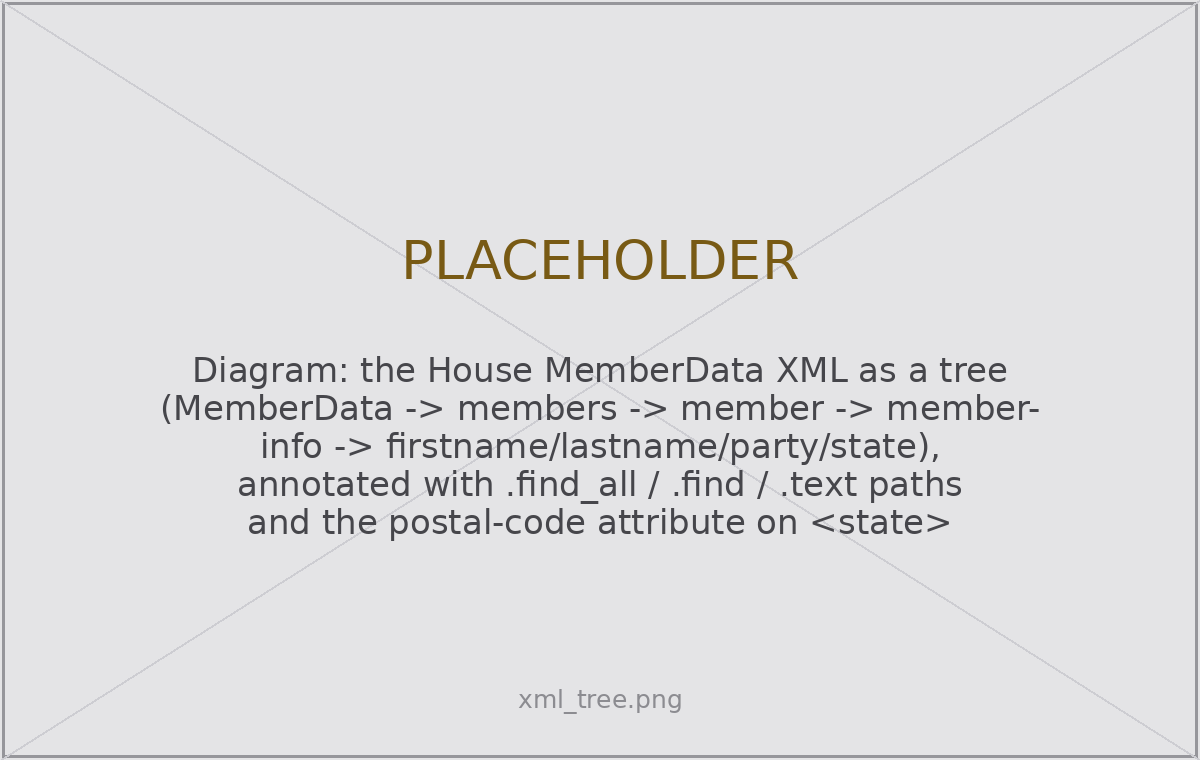
\includegraphics[width=\textwidth]{img/xml_tree.png}\\
            {\scriptsize The House \texttt{MemberData} feed, drawn as a tree.}
        \end{column}
    \end{columns}
    \bottomcite{Textbook Ch.~4, ``The Tree Structure.'' The siblings-with-HTML idea returns in Ch.~6.}
\end{frame}

\begin{frame}{JSON: lists and dictionaries you already know}
    \begin{columns}[T]
        \begin{column}{0.54\textwidth}
            JSON maps onto two Python structures you already use:
            \begin{itemize}\small
                \item a JSON \textbf{array} is a Python \textbf{list} --- ordered, indexed by position
                \item a JSON \textbf{object} is a Python \textbf{dict} --- accessed by key
            \end{itemize}

            \vspace{0.75em}
            Real data \textbf{nests} them --- dicts inside lists inside dicts, several levels deep. The skill is navigating from the outside in, one key or index at a time.

            \vspace{0.75em}
            {\footnotesize Created by Douglas Crockford in the early 2000s; the rise of AJAX made JSON the default API format by the 2010s.}
        \end{column}
        \begin{column}{0.42\textwidth}
            \centering
            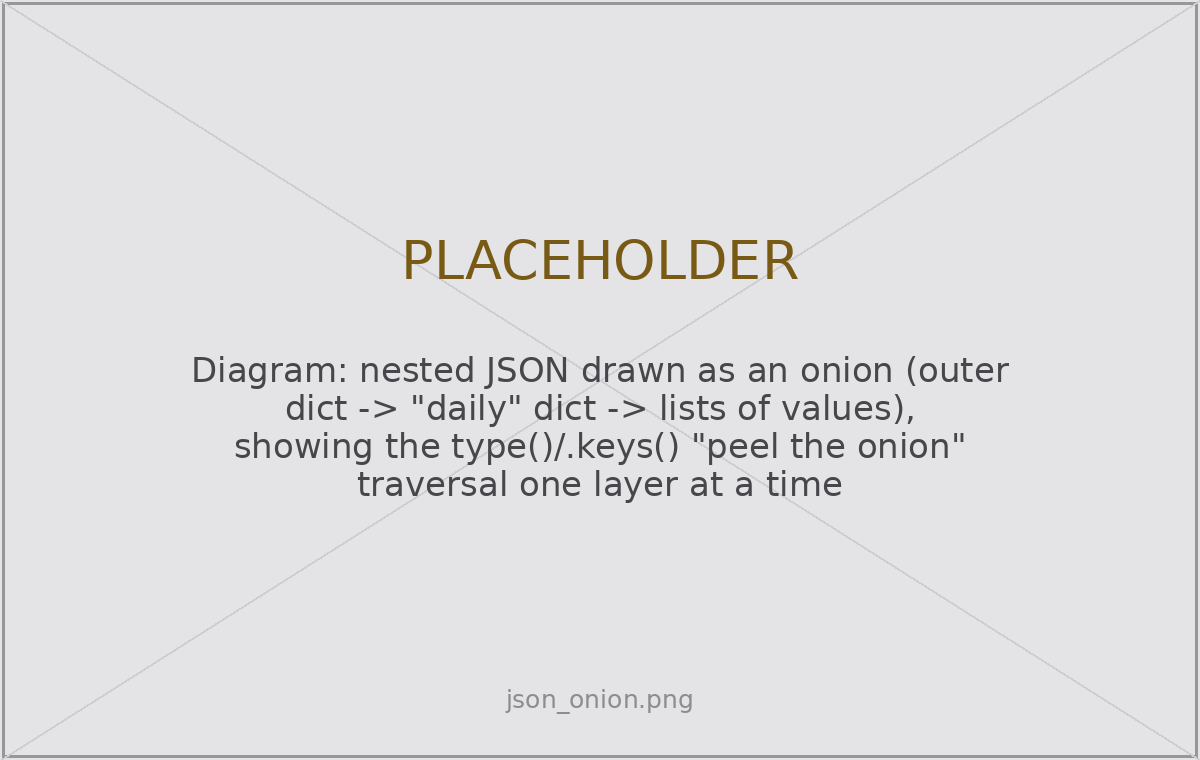
\includegraphics[width=\textwidth]{img/json_onion.png}\\
            {\scriptsize ``Peel the onion'': \texttt{type()}, then \texttt{.keys()}, one layer deeper each time.}
        \end{column}
    \end{columns}
    \bottomcite{Textbook Ch.~4, ``JSON and Python Data Structures.''}
\end{frame}

\begin{frame}{One pipeline unifies the whole course}
    \begin{columns}[T]
        \begin{column}{0.58\textwidth}
            Whether data starts as XML, JSON, HTML, or PDF text, the move into analysis is always the same:

            \vspace{0.6em}
            \begin{center}
                \textbf{find records} $\rightarrow$ \textbf{extract fields} $\rightarrow$\\[0.2em] \textbf{list of dictionaries} $\rightarrow$ \texttt{pd.DataFrame}
            \end{center}

            \vspace{0.6em}
            The DataFrame is the \textbf{universal intermediate format}. Reach it and all of pandas opens up: filter, group, cross-tabulate, merge.

            \vspace{0.6em}
            The source changes; the tag names change; \textbf{the pipeline stays the same}.
        \end{column}
        \begin{column}{0.38\textwidth}
            \begin{block}{You reuse this pattern in\dots}
                \footnotesize
                \begin{itemize}\footnotesize
                    \item HTML tables --- Ch.~6
                    \item archived pages --- Ch.~7
                    \item PDF text --- Ch.~9
                    \item Wikipedia, government \& social APIs --- Ch.~10--12
                \end{itemize}
            \end{block}
        \end{column}
    \end{columns}
    \bottomcite{Textbook Ch.~4, ``From XML to DataFrame.'' The same pattern recurs in every later chapter.}
\end{frame}

% =========================================================================
\section{Wednesday · Notebook Lab}
% =========================================================================

\begin{frame}[fragile]{Wednesday --- parsing XML with BeautifulSoup}
    Parse the string into a navigable tree, then search it. \texttt{.find()} returns the first match, \texttt{.find\_all()} returns them all --- each searches the \textit{entire} subtree beneath a tag:
\begin{lstlisting}
from bs4 import BeautifulSoup

soup = BeautifulSoup(house_raw, "xml")   # the "xml" parser comes from lxml

members = soup.find_all("member")
print(len(members))                       # 2

for m in members:
    first = m.find("firstname").text      # .text = content between the tags
    last  = m.find("lastname").text       # .find() reaches nested tags too
    party = m.find("party").text
    print(f"{first} {last} ({party})")    # Joe Neguse (D) / Jeff Hurd (R)
\end{lstlisting}
    \bottomcite{Textbook Ch.~4, ``Parsing with BeautifulSoup.'' Hyphenated names like \texttt{member-info} break dot-notation --- use \texttt{.find()}.}
\end{frame}

\begin{frame}[fragile]{The two-place problem --- and the crash that guards it}
    \begin{columns}[T]
        \begin{column}{0.54\textwidth}
            A value is either \textbf{text} or an \textbf{attribute}:
\begin{lstlisting}
state = soup.find("state")
state["postal-code"]                # "CO"
state.find("state-fullname").text   # "Colorado"
\end{lstlisting}
            A missing tag makes \texttt{.find()} return \texttt{None}:
\begin{lstlisting}
# AttributeError: None has no .text
m.find("party").text
# guard every extraction instead:
m.find("party").text if m.find("party") else None
\end{lstlisting}
        \end{column}
        \begin{column}{0.44\textwidth}
            Working out \textit{which} of the two holds your value is half the parsing battle --- real XML uses both.

            \vspace{0.75em}

            Calling \texttt{.text} on a \texttt{None} is the \textbf{single most common} scraping error. The \texttt{if \dots else None} guard keeps one missing field from crashing a 441-record loop.

            \vspace{0.75em}

            XML always hands you \textbf{text}: converting \texttt{"2nd"} or \texttt{"\$1,234"} to a number is your job.
        \end{column}
    \end{columns}
    \bottomcite{Textbook Ch.~4, ``Parsing with BeautifulSoup'' \& ``Common Issues to Debug.''}
\end{frame}

\begin{frame}[fragile]{XML $\rightarrow$ DataFrame: the real House roster}
    \begin{columns}[T]
        \begin{column}{0.6\textwidth}
\begin{lstlisting}
import requests, pandas as pd

url = "https://clerk.house.gov/xml/lists/MemberData.xml"
soup = BeautifulSoup(requests.get(url).text, "xml")
print(soup.find("MemberData")["publish-date"])

records = []
for m in soup.find_all("member"):    # 441 members
    st = m.find("state")
    records.append({"last_name": m.find("lastname").text,
                    "party": m.find("party").text,
                    "state": st["postal-code"] if st else None})
df = pd.DataFrame(records)   # find_all -> dicts -> DataFrame
\end{lstlisting}
        \end{column}
        \begin{column}{0.36\textwidth}
            \centering
            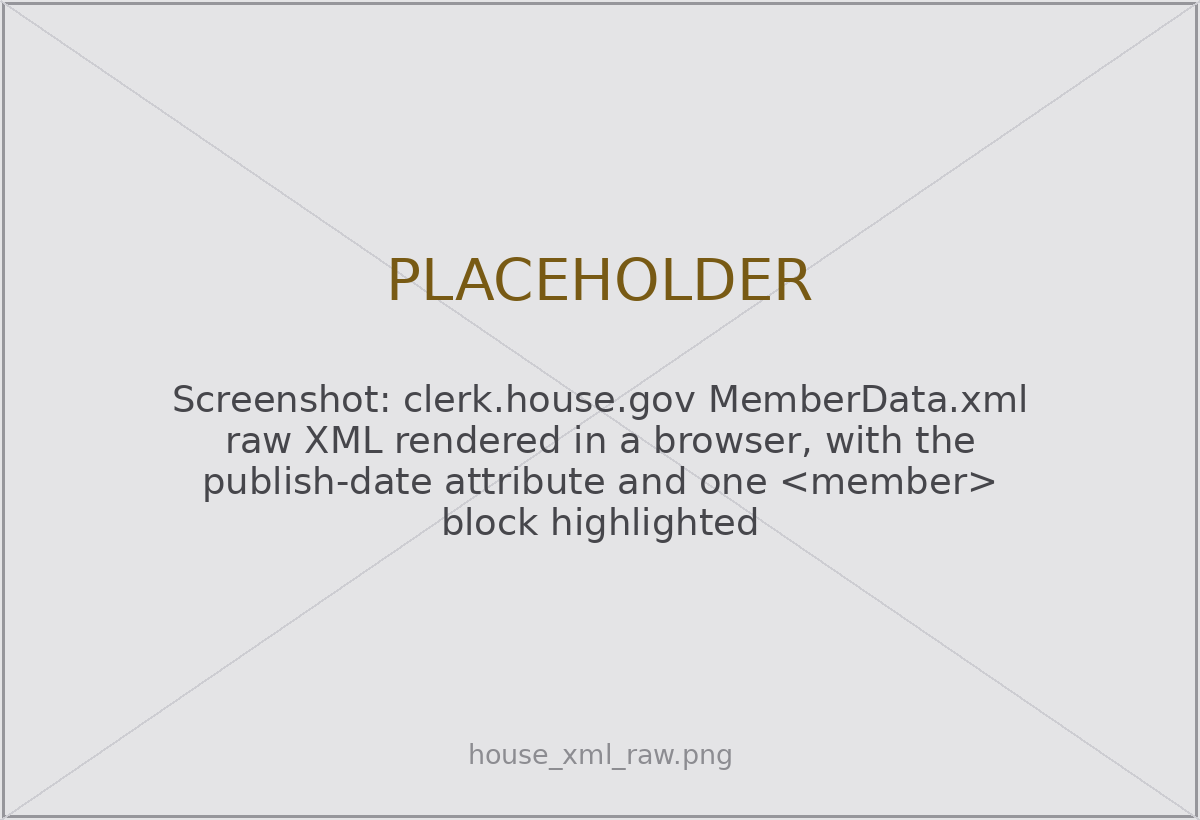
\includegraphics[width=\textwidth]{img/house_xml_raw.png}\\
            {\scriptsize The Clerk's live \texttt{MemberData.xml}.}
        \end{column}
    \end{columns}
    \bottomcite{Textbook Ch.~4, ``From XML to DataFrame.'' 441 = 435 voting members + 6 delegates; record the \texttt{publish-date}.}
\end{frame}

\begin{frame}[fragile]{JSON: parse a string, then the list-of-dictionaries pipeline}
    \texttt{json.loads()} turns a \textbf{s}tring into Python objects (\texttt{json.load()} reads a \textbf{f}ile). With \texttt{requests}, \texttt{response.json()} does it for you:
\begin{lstlisting}
import json, pandas as pd

data = json.loads('{"state": "Colorado", "population": 5773714}')
print(data["state"])              # Colorado
# response.json()  ==  json.loads(response.text)

census = [                        # the list-of-dictionaries pattern:
    {"state": "Colorado", "year": 2020, "population": 5773714},
    {"state": "Colorado", "year": 2010, "population": 5029196},
]
df = pd.DataFrame(census)         # one dict per row, keys -> columns
\end{lstlisting}
    \bottomcite{Textbook Ch.~4, ``Parsing JSON Strings'' \& ``The List-of-Dictionaries Pattern.''}
\end{frame}

\begin{frame}[fragile]{JSON: peel the onion on a live API}
    \begin{columns}[T]
        \begin{column}{0.58\textwidth}
\begin{lstlisting}
import requests

url = "https://api.open-meteo.com/v1/forecast"
params = {"latitude": 40.01, "longitude": -105.27,
          "daily": "temperature_2m_max",
          "timezone": "America/Denver"}
data = requests.get(url, params=params).json()

# type() + .keys(), one level deeper each time
data.keys()            # latitude, longitude, daily...
data["daily"].keys()   # time, temperature_2m_max
highs = data["daily"]["temperature_2m_max"]  # a list
data.get("elevation", "unknown")  # .get avoids KeyError
\end{lstlisting}
        \end{column}
        \begin{column}{0.4\textwidth}
            \centering
            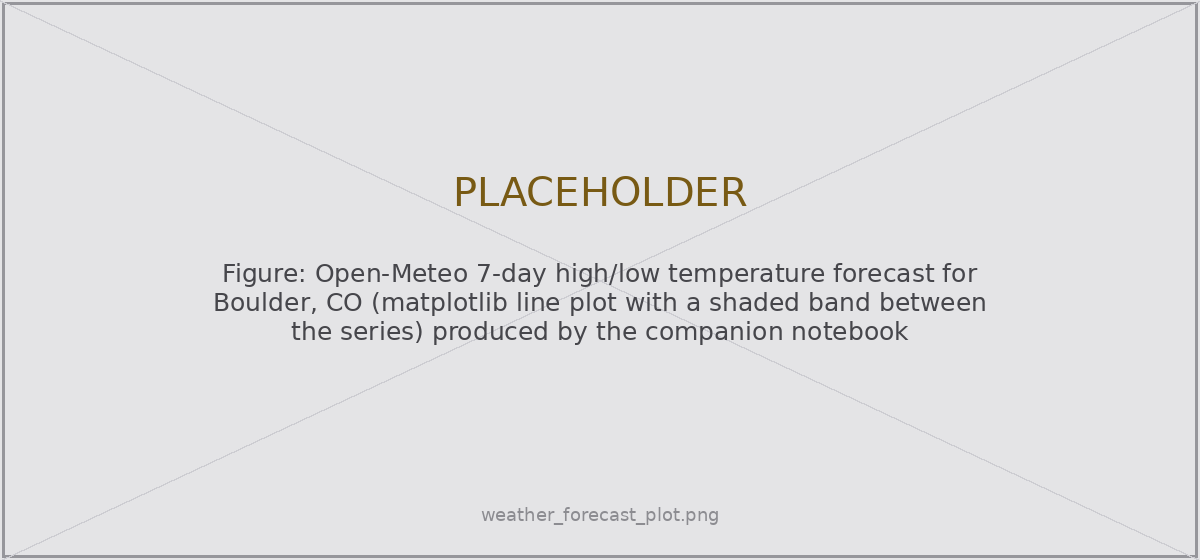
\includegraphics[width=\textwidth]{img/weather_forecast_plot.png}\\
            {\scriptsize Boulder's 7-day forecast, straight from the nested lists.}
        \end{column}
    \end{columns}
    \bottomcite{Textbook Ch.~4, ``Handling Deeply Nested JSON.'' \texttt{.get(key, default)} returns a default instead of raising \texttt{KeyError}.}
\end{frame}

\begin{frame}{Lab: work these in pairs, then show-and-tell}
    \begin{columns}[T]
        \begin{column}{0.62\textwidth}
            From the Chapter 4 notebook:
            \begin{enumerate}\small
                \item \textbf{RSS feed} --- parse a news feed with the \texttt{"xml"} parser; pull title, link, pubDate $\rightarrow$ DataFrame
                \item \textbf{Nested JSON} --- Open-Meteo dates + max temps $\rightarrow$ DataFrame
                \item \textbf{XML vs.\ JSON} --- same data, both formats: which parses easier? which carries more metadata?
                \item \textbf{Reusable} --- write \texttt{xml\_to\_dataframe(soup, tag, fields)}; test on Congress, then an RSS feed
                \item \textbf{Weather} --- plot high \& low temperatures; flag days that drop below freezing
                \item[6.] \textcolor{tab-purple}{\textbf{5617}}: a datasheet-style critique of a public XML/JSON dataset (\textcite{gebru2021datasheets})
            \end{enumerate}
        \end{column}
        \begin{column}{0.34\textwidth}
            \begin{block}{Show-and-Tell}
                \footnotesize Come ready to share:
                \begin{itemize}\footnotesize
                    \item a challenging bug
                    \item interesting data you pulled
                    \item a provocation for a research design
                \end{itemize}
            \end{block}
        \end{column}
    \end{columns}
\end{frame}

\begin{frame}[standout]
    The data source changes.\\
    The tag names change.\\
    The pipeline stays the same.\\[1em]
    {\large \texttt{find\_all} $\rightarrow$ dicts $\rightarrow$ \texttt{DataFrame}.}
\end{frame}

% =========================================================================
\section{Friday · Textbook Revisions}
% =========================================================================

\begin{frame}{Friday --- improving Chapter 4 together}
    \begin{columns}[T]
        \begin{column}{0.6\textwidth}
            Today we make the book better. Each of you opens a \textbf{pull request} against \texttt{ch-04-data-formats.qmd} and reviews a classmate's.

            \vspace{1em}
            The workflow (from Week 1):
            \begin{enumerate}\small
                \item Branch / fork the book repo
                \item Edit the chapter; commit with a clear message
                \item Open a PR describing \textit{what} and \textit{why}
                \item Review two peers' PRs: kind, specific, actionable
            \end{enumerate}
        \end{column}
        \begin{column}{0.36\textwidth}
            \centering
            
\includegraphics[width=\textwidth]{img/pr_review.png}
        \end{column}
    \end{columns}
    \bottomcite{Contributions \& reviews count toward the Textbook Revisions grade (30\%).}
\end{frame}

\begin{frame}{A revision menu for Chapter 4}
    High-value targets --- pick one and scope it to a single PR:
    \begin{itemize}
        \item \textbf{Test the code against live sources.} The House roster drifts (441 today; the \texttt{publish-date} changes) and Open-Meteo dates roll forward. Run the notebook, report what changed, and pin the snapshot.
        \item \textbf{Close a gap in ``Common Issues to Debug.''} Add a worked \texttt{json.JSONDecodeError} case --- a trailing comma, single quotes, or an HTML error page returned instead of JSON.
        \item \textbf{Add a figure.} The chapter has \textit{no} diagrams: contribute a clean XML-tree or a JSON ``peel-the-onion'' figure.
        \item \textbf{Strengthen an exercise.} Give the RSS or weather exercise expected output, a rubric, or a starter cell so it is self-checking.
        \item \textbf{Extend the RSS / post-API story.} Tie the decline-of-RSS narrative to a concrete citation and the ``soft enclosure'' theme (Ch.~3).
    \end{itemize}
    \bottomcite{Targets drawn from the chapter's callouts, ``Common Issues,'' exercises \& ``Further Reading.''}
\end{frame}

\begin{frame}{What makes a good revision \& a good review}
    \begin{columns}[T]
        \begin{column}{0.48\textwidth}
            \begin{block}{A strong PR}
                \begin{itemize}\small
                    \item One focused change, clearly titled
                    \item Explains the problem it fixes
                    \item Renders (\texttt{quarto render}) without errors
                    \item Matches the book's voice and notation
                    \item Discloses any AI assistance
                \end{itemize}
            \end{block}
        \end{column}
        \begin{column}{0.48\textwidth}
            \begin{block}{A strong review}
                \begin{itemize}\small
                    \item Runs / reads the change, not just skims
                    \item Names specifics (line, claim, code)
                    \item Separates ``must fix'' from ``nice to have''
                    \item Is generous --- assume good faith
                    \item Ends with a clear verdict
                \end{itemize}
            \end{block}
        \end{column}
    \end{columns}
    \vspace{0.5em}
    \centering\small Next week: \textbf{Web Architecture \& Protocols} --- how a URL becomes a rendered page (HTTP, requests, status codes).
\end{frame}

% =========================================================================
\begin{frame}{Key takeaways}
    \begin{enumerate}
        \item \textbf{XML} is a tree of tags; \textbf{JSON} is nested lists and dictionaries --- the two structural languages of web data.
        \item BeautifulSoup navigates XML with \texttt{.find()}, \texttt{.find\_all()}, and \texttt{.text}; attributes come out with bracket notation.
        \item For JSON, \textbf{peel the onion} --- inspect \texttt{type()} and \texttt{.keys()} top-down, and use \texttt{.get()} for safe access.
        \item The \texttt{find\_all} $\rightarrow$ list-of-dicts $\rightarrow$ \texttt{DataFrame} pipeline is the bridge from raw web data to analysis.
        \item Format is a \textbf{transparency} choice: open XML/JSON serves public oversight; scanned PDFs quietly enclose it.
    \end{enumerate}
    \vspace{0.75em}
    \bottomcite{Reading: Textbook Ch.~4. Related: \textcite{mitchell2018web}; \textcite{vandenbroucke2018practical}.}
\end{frame}

\end{document}
